\subsection{Principi di design}
La piattaforma è organizzata in moduli relazionati tra loro prestando attenzione
alla creazione di componenti coesi, disaccoppiati e che rispettino i principi SOLID.
Un modulo esiste per incapsulare dei servizi che vengono erogati attraverso dei componenti
che collaborano per portare a termine il compito richiesto. Ciascuno di essi può definire i moduli da importare per sfruttarne i servizi, i controller da esporre per gestire le richieste e i servizi che esporta.
Di conseguenza un modulo espone una interfaccia software costituita dai servizi che esporta e una interfaccia REST costituita dagli endpoint, definiti nei controller esposti,
che permettono di interagire con l'applicazione attraverso richieste HTTP.

Nella piattaforma avremo i seguenti moduli funzionali:
\begin{itemize}
    \itemsep0em
    \item Auth Module: si occupa di tutti gli aspetti inerenti alla autenticazione e autorizzazione degli utenti.
    \item User Module: si occupa della gestione delle informazioni degli utenti.
    \item Demo Module: permette la registrazione a servizi in versione demo.
    \item Mail Module: permette di gestire le richieste di invio email al \textit{message broker}.
\end{itemize}
Ognuno di questi moduli è organizzato con una architettura a tre strati (vedi Figura \ref{fig:three-tier}) così definita:
\begin{itemize}
    \itemsep0em
    \item Controller Layer: contiene gli elementi, detti controllers, che permettono all'utente di interagire con i servizi offerti dalla piattaforma.
    \item Service Layer: contiene gli elementi, detti services, che hanno il compito di elaborare i dati (business logic).
    \item Data Access Layer: contiene gli elementi, detti models, che permettono di interagire con il database.
\end{itemize}

I moduli, i controller e i servizi sono delle istante \textit{singleton}, create
all'avvio dell'applicazione e condivise al suo interno. Inoltre ogni componente sfrutta il meccanismo
della \textit{dependency injection} per risolvere le proprie dipendenze e ciò comporta
notevoli vantaggi per quando riguarda la riusabilità del codice e la verifica del comportamento dei componenti
nella fase di test.
Nella applicazione sarà poi presenta anche un modulo di \textit{root}, detto \textit{application module}, che
permette si risolvere le dipendenze tra i vari elementi della applicazione e ne esegue l'avvio.
Inoltre ogni modulo potrà poi essere convertito in microservizio nel caso in cui si voglia avere la possibilità di scalare
indipendentemente i vari servizi in base alle esigenze richieste dalle operazioni degli utenti.
Questi elementi supportano la realizzazione di una architettura scalabile, coesa, disaccoppiata e mantenibile.

\begin{figure}[H]
    \centering
    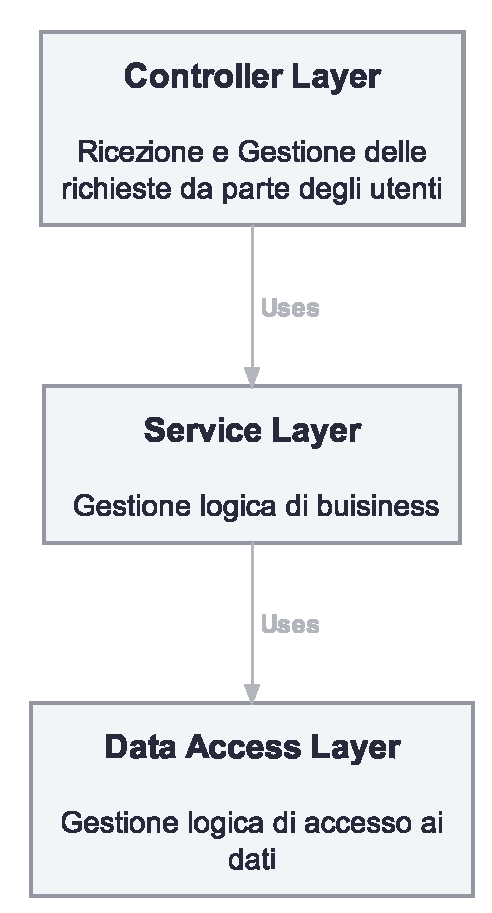
\includegraphics[scale=0.5]{three-tier.eps}
    \caption{Schema riassuntivo della architettura \textit{three-tier}}
    \label{fig:three-tier}
\end{figure}